\partabstractfp{\textbf{This is the abstract of this part}. \lipsum[10]}
\partabstractrp{\lipsum[11]}
\partabstractlettrine{A}{bstract} % the first word of the abstract

\part{}

\chapter{Tables and figures}
\section{(title section 1)}
\subsection{(title sub-section 1)}



\textbf{This is an example of a wide figure (odd pages).}
\begin{figure*}[!htbp]
  \wdfigbox
  {\caption{Bundling creates a complex security}}
  {
  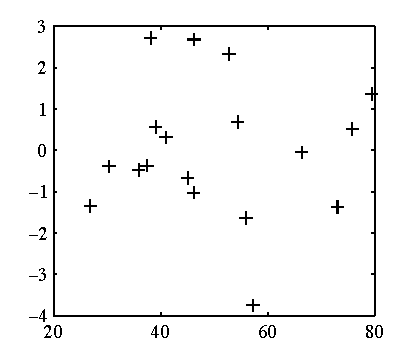
\includegraphics{./figure/sample.pdf}
  \floatfoot{Source: \textit{The Wall Street Journal}, December 19, 2001}
  }
\end{figure*}

\lipsum[7-8]

\textbf{This is an example of a wide figure (even pages).}
\begin{figure*}[!htbp]
  \wdfigbox
  {\caption{Bundling creates a complex security}}
  {
  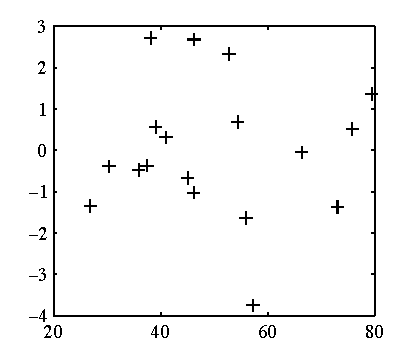
\includegraphics{./figure/sample.pdf}
  \floatfoot{Source: \textit{The Wall Street Journal}, December 19, 2001}
  }
\end{figure*}


\subsection{(title sub-section 2)}

\lipsum[1]
\tmarginpar{Margin note title}{This is a margin note, This is a margin note, This is a margin note}
\lipsum[2-5]

\section{(title section 2)}

\lipsum[1]
\tmarginpar{Margin note title}{This is a margin note, This is a margin note, This is a margin note}
\lipsum[2-5]

\subsection{(title sub-section 1)}

\lipsum[1-4]
\tmarginpar{Margin note title}{This is a margin note, This is a margin note, This is a margin note}
\lipsum[5]

\subsection{(title sub-section 2)}

\lipsum[1]
\lipsum[2-5]

\chapter{Other environments}
\section{(title section 1)}
\subsection{(title sub-section 1)}

\lipsum[9]

\textbf{This is a new example environment, you can define other similar environment in the similar way.}
\begin{example*}
  \wdexpbox
  {\caption{Bundling creates a complex security}}
  {\lipsum[10]}
\end{example*}
\newpage
\lipsum[11]

\begin{example*}
  \wdexpbox
  {\caption{Bundling creates a complex security}}
  {\lipsum[12]}
\end{example*}

\subsection{(title sub-section 2)}
\section{(title section 2)}
\subsection{(title sub-section 1)}
\subsection{(title sub-section 2)}

\partabstractfp{\lipsum[12]}
\partabstractrp{\lipsum[13]}
\partabstractlettrine{B}{bstract}

% those bunch of chapters and sections are only used for filling the table of contents :P
\part{QUESTIONS OF TECHNIQUE}
\chapter{Chapter 1}
\section{(title section 1)}
\subsection{(title sub-section 1)}
\subsection{(title sub-section 2)}
\section{(title section 2)}
\subsection{(title sub-section 1)}
\subsection{(title sub-section 2)}
\chapter{Chapter 2}
\section{(title section 1)}
\subsection{(title sub-section 1)}
\subsection{(title sub-section 2)}
\section{(title section 2)}
\subsection{(title sub-section 1)}
\subsection{(title sub-section 2)}
\chapter{Chapter 3}
\section{(title section 1)}
\subsection{(title sub-section 1)}
\subsection{(title sub-section 2)}
\section{(title section 2)}
\subsection{(title sub-section 1)}
\subsection{(title sub-section 2)}
\chapter{Chapter 4}
\section{(title section 1)}
\subsection{(title sub-section 1)}
\subsection{(title sub-section 2)}
\section{(title section 2)}
\subsection{(title sub-section 1)}
\subsection{(title sub-section 2)}
\chapter{Chapter 5}
\section{(title section 1)}
\subsection{(title sub-section 1)}
\subsection{(title sub-section 2)}
\section{(title section 2)}
\subsection{(title sub-section 1)}
\subsection{(title sub-section 2)}
\chapter{Test of large page numbers}
\section{(title section 1)}
\subsection{(title sub-section 1)}
\subsection{(title sub-section 2)}
\section{(title section 2)}
\setcounter{page}{1000}
\subsection{(title sub-section 1)}
\textbf{This is a test for large page numbers. Note that the header for titles remains the same location even if the page number is large.}

\subsection{(title sub-section 2)}

\textattachfile{symbols.pdf} % 这里加入所添加的附件
%%% Local Variables: 
%%% TeX-master: "book_template_2"
%%% End: 
